
\section{Evaluation: Does Skill Distance Predict Selection?}\label{sec:evaluation_skill_distance}

This section evaluates whether our job postings based skill-distance measure meaningfully captures skill requirements by testing how well 
our derived distance metric predicts selection of internal candidates for new positions. Our primary interest lies in understanding the 
extent to which posting content predicts selection, and in assessing the relative contribution of the skill distance measure compared to 
a few other observed features. While an Area Under the Curve (AUC) of 0.62 might appear modest in a traditional classification setting, 
the key contribution of this section is demonstrating the surprisingly rich and informative signal captured by a distance metric derived 
solely from job posting content. Even with this level of predictive power, we reveal that job postings contain substantial information 
about the skills relevant to selection decisions.

Our test set comprises 308 cases where internal applicants applied to vacancies (approximately 25\% of our total cases). 
We examine whether skill distances computed purely from posting content capture predictable variation in selection outcomes. 
It's important to note that the information contained in an applicant's job description ($j_c$) may not fully capture the skills 
and abilities of that position, let alone those of the candidate. This potential measurement loss informs our approach.
 

\subsection{Skill Distance and Selection Probability}

To assess the relationship between skill distance and selection probability, we employ a logistic regression to quantify the association:

\begin{equation}
\text{logit}(P(\text{S}{c,v} = 1)) = \beta_0 + \beta_1 \times Q_k(d{j_c, j_v})
\end{equation} 

Here, \( Q_k(d_{j_c, j_v}) \) represents the quintile of the skill distance between the applicant's current job (\( j_c \)) and the vacancy (\( j_v \)). We discretize the 
distance into a categorical variable, as the relationship between selection probability and distance is unlikely to be simply linear. This discretization offers stability 
and robustness to extreme values while retaining easy interpretation. \autoref{tab:logistic_regression} shows that the coefficient for skill distance is negative and 
significant \((\beta_1 = -0.3268, \, p < 0.01)\), indicating that applicants with lower skill distance to a vacancy have a higher likelihood of being selected.


\begin{table}[h]
    \centering
    \caption{Logistic Regression Results for Skill Distance and Selection Probability}
    \renewcommand{\arraystretch}{1.2} 
    \begin{tabular}{lcc}
    \hline
    \textbf{Variable} & \textbf{Coefficient} & \textbf{Std. Error} \\
    \hline
    Intercept & 1.1171*** & 0.265 \\
    Quintile & -0.3268*** & 0.086 \\
    \hline
    Observations & \multicolumn{2}{c}{308} \\
    Pseudo R-squared & \multicolumn{2}{c}{0.03551} \\
    \hline
    \multicolumn{3}{l}{\footnotesize{*** p$<$0.01}} \\
    \end{tabular}
    \label{tab:logistic_regression}
\end{table}

The regression suggests that, on average, an applicant-vacancy pair in the lowest skill distance quintile has an 84\% 
higher probability of selection compared to a pair in the highest quintile. This substantial difference in selection 
probability across skill distance quintiles strongly suggests that our posting-derived metric is effectively capturing 
informative variations in the skill alignment between applicants and vacancies.


\begin{figure}[h]
    \centering
    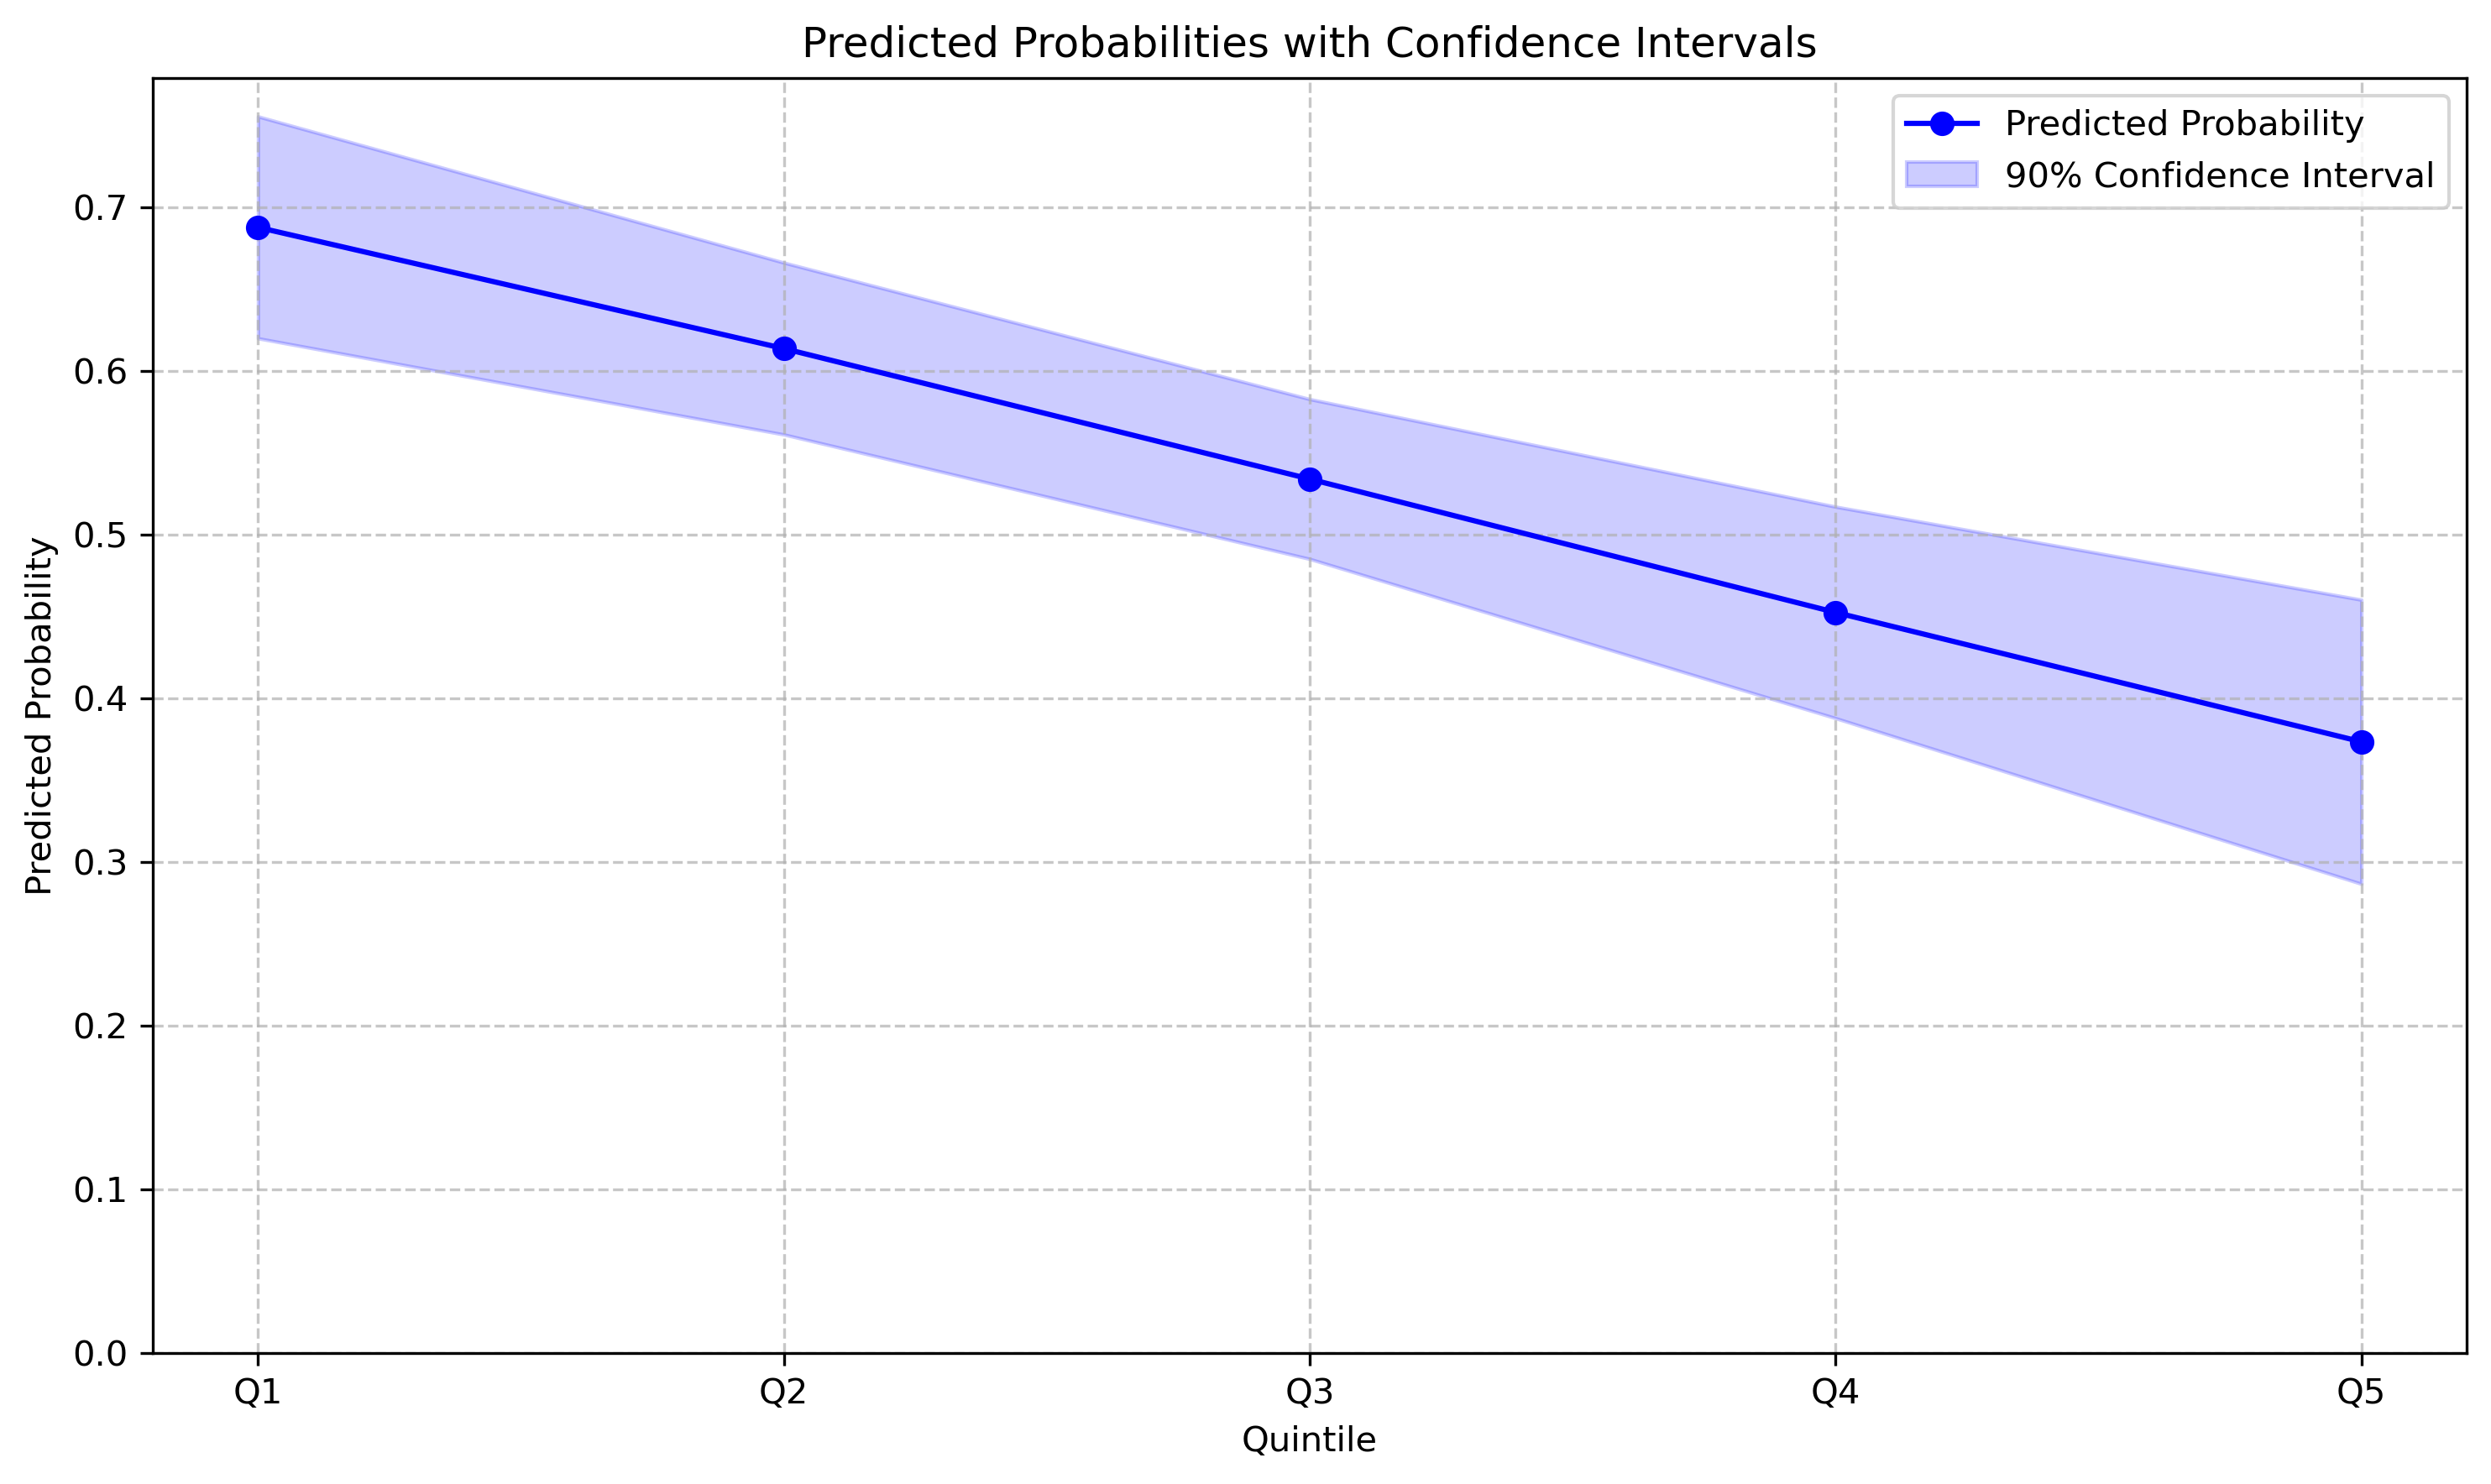
\includegraphics[width=0.75\textwidth]{new_img/pp.png}
    \caption{Selection Probability by Skill Distance Quintile}
    \label{fig:skill_distance_probability}
\end{figure}

While skill distance accounts for a small component of the variation in selection decisions, its ability to capture differences in selection probability is unambiguous. 
We will now exploit the structure in our test sample to examine the association. 


\subsection{Skill Distance: Within-Vacancy and Within-Applicant Variation}

When multiple internal candidates apply to the same vacancy, we have an opportunity to verify if selection among different applicants for the same position is predicted 
by their respective skill distances. Correlation between skill distance and selection measured at each vacancy level would convey a more direct link of the measured distance. 
Similarly, we have cases where an applicant has applied to different vacancies. This allows us to focus on applicant-level selection data to examine whether the applicant 
has a higher selection probability for vacancies to which they have a low skill distance. Focusing on a single applicant allows us to control for unobserved factors that 
influence their selection chances across vacancies, such as broadly relevant skills they have acquired or performance in their current job. While we have already established 
a notable negative association between skill distance and selection, these analyses would further demonstrate that the measured skill distance captures significant selection 
variation at both the applicant and vacancy levels, thereby reinforcing the measure's informativeness.



\subsubsection{Within-Vacancy Selection}

To assess the predictive power of the skill distance metric, we evaluated the proportion of vacancies where the applicant with the lowest skill distance was selected. Our 
analysis encompassed 261 observations across 110 vacancy groups from our test set, each group comprising a vacancy with multiple internal applicants and one selection. The 
analysis revealed that the candidate with the lowest skill distance was chosen in 69.92\% of cases, suggesting the metric's reliability in predicting selection outcomes. We 
further analyzed the role of skill distance in the selection probability among applicants competing for the same vacancy using a conditional logit model. The model incorporated 
vacancy-specific fixed effects ($\alpha_v$) to concentrate on within-vacancy variation. The results indicated that being in a higher skill distance quintile decreased the 
probability of selection by 35\% ($\beta = -0.4293$, $p < 0.01$). The initial exploratory analysis demonstrates the skill distance metric's capacity to predict selection 
outcomes in a majority of cases. Building on this, the more formal conditional logit model enables a rigorous examination of the role of skill distance in differentiating 
applicants within the same vacancy. Together, these findings highlight the relevance and importance of the skill distance measure in the selection process. 

\begin{equation}
\text{logit}(P(\text{S}_{v,c} = 1)) = \alpha_v + \beta Q_k(d_{j_c,j_v})
\end{equation}

\begin{table}[h]
    \centering
    \caption{Conditional Logit Model Results for Within-Vacancy Analysis}
    \renewcommand{\arraystretch}{1.2}
    \begin{tabular}{lcc}
    \hline
    \textbf{Variable} & \textbf{Coefficient} & \textbf{Std. Error} \\
    \hline
    Quintile & -0.4293*** & 0.122 \\
    \hline
    Observations & \multicolumn{2}{c}{261} \\
    Groups & \multicolumn{2}{c}{110} \\
    \hline
    \multicolumn{3}{l}{\footnotesize{*** p$<$0.01}} \\
    \end{tabular}
    \label{tab:within_vacancy}
\end{table}



These results underscore the relevance and importance of the skill distance measure in the selection process. 
Crucially, the ability of skill distance to differentiate between candidates applying for the same position highlights 
the fine-grained informativeness embedded within job postings regarding the specific requirements of that role.

\subsubsection{Within Applicant Selection}

Now, we analyze the ability of our skill distance measure to account for selection decisions within an applicant's multiple vacancies. We again employ a conditional logit model, 
this time incorporating applicant-specific fixed effects ($\alpha_c$).


\begin{equation}
\text{logit}(P(\text{S}_{c,v} = 1)) = \alpha_c + \beta Q_k(d_{j_c,j_v})
\end{equation}

The test dataset now comprises 111 observations from 33 applicant groups, each applying to multiple vacancies. The results reveal that applicants in higher skill distance 
quintiles experience a 50\% reduction in selection probability (\(\beta = -0.695\), \(p = 0.017\)). This demonstrates that the measured skill distance effectively accounts 
for selection decisions within applicants. 


\begin{table}[h]
    \centering
    \caption{Conditional Logit Model Results for Across-Applicant Analysis}
    \renewcommand{\arraystretch}{1.2}
    \begin{tabular}{lcc}
    \hline
    \textbf{Variable} & \textbf{Coefficient} & \textbf{Std. Error} \\
    \hline
    Quintile & -0.695** & 0.290 \\
    \hline
    Observations & \multicolumn{2}{c}{111} \\
    Groups & \multicolumn{2}{c}{33} \\
    \hline
    \multicolumn{3}{l}{\footnotesize{** p$=$0.017}} \\
    \end{tabular}
    \label{tab:across_applicant}
\end{table}


These patterns demonstrate that the skill distance from an applicant's current job provides valuable information for predicting selection to new internal vacancies. While 
selection typically depends on an applicant's skill-set and preparedness for the new position's demands, our findings reveal that a distance measure constructed from job 
postings and past selection decisions correlates strongly with observed selection patterns. This correlation opens an analytical window into the firm, linking skills to 
internal mobility. Before exploring these links we examine how important is the skill distance measure relative to other observed features in predicting selection to vacancies.



\subsection{Other Observed Features}

While our paper primarily focuses on leveraging information from job postings and selection decisions, we recognize the importance of evaluating other predictors of 
internal candidate selection. To enhance our understanding of selection patterns, we examine additional features available in the firm's information system. We compare 
the performance of our skill distance metric against other observed applicant characteristics, including tenure at the organization, total work experience, job category, 
vacancy (job sought) category, and proficiency rating. Table \ref{tab:other_features} presents summary statistics for these features. 

\begin{table}[h]
    \centering
    \caption{Summary Statistics -- Other Observed Features}
    \begin{tabular}{l c c c c}
        \toprule
        \textbf{Notation} & \textbf{Description} & \textbf{Unit} & \textbf{25th Percentile} & \textbf{75th Percentile} \\
        \midrule
        $t_c$ & Tenure at $c$ & days & 661 & 1346 \\
        $T_c$ & Total experience & days & 1927 & 3009 \\
        $l_c$ & Job category & 4 levels & 2 & 3 \\
        $l_v$ & Vacancy category & 4 levels & 2 & 3 \\
        $p_c$ & Proficiency rating & 4 levels & 2 & 2 \\
        \bottomrule
    \end{tabular}
    \label{tab:other_features}
\end{table}

The data shows notable differences among applicants. Tenure ranges from about 2 years to 3.5 years, while total experience spans from roughly 5 years to 8 years at the 25th and 75th percentiles. Job and vacancy categories both range from level 2 to 3, indicating movement across organizational tiers. Proficiency ratings, however, remain consistent at level 2 for at the 25th and 75th percentiles. These observed features, as shown in Table \ref{tab:other_features}, display clear variation across the applicant pool. Their potential to explain selection patterns merits further exploration, complementing our primary skill distance metric.


To assess the relative importance of the skill distance measure  we employ Random Forest classifiers. The well known ensemble learning algorithm captures complex interactions between variables. We train two Random Forest models on our training dataset: one incorporates all features including skill distance, while the other excludes skill distance. This method isolates and quantifies the predictive power of the skill distance metric relative to other observed features. We evaluate these models on our test set and will again employ the AUC metric. Table \ref{tab:model_comparison} presents the AUC scores for both models on the test set.

\begin{table}[h]
    \centering
    \caption{Model Comparison: Random Forest Classifiers with and without Skill Distance}
    \renewcommand{\arraystretch}{1.2} 
    \begin{tabular}{lcc}
    \hline
    \textbf{Model} & \textbf{AUC Score} \\
    \hline
    Full Model (with Skill Distance) & 0.600 \\
    Model without Skill Distance & 0.500 \\
    \hline
    \end{tabular}
    \label{tab:model_comparison}
\end{table}




The full model, which includes skill distance, achieves an AUC of 0.600, while the model without skill distance yields an AUC of 0.500 - equivalent to 
a classifier with no predictive ability. This dramatic difference in performance powerfully illustrates the substantial informative content captured by 
the skill distance measure. Despite the clear variation in other observed features such as tenure, total experience, job categories, and proficiency 
ratings, skill distance alone accounts for nearly all predictable variation in selection outcomes.

This finding is particularly noteworthy given that we derived our measure from job descriptions, which are generally less sensitive than other HR data. 
While firms often possess additional potentially predictive features, these may be subject to privacy concerns or legal restrictions. Our approach demonstrates 
that valuable insights can be derived from less sensitive data sources, advancing the field of people analytics while maintaining ethical data practices. Moreover, 
the granularity of our skill distance measure appears to capture nuanced differences between roles that categorical variables like performance ratings may miss, 
especially when applicants cluster in just one or two groups.